\documentclass{article}
\usepackage{enumerate}
\usepackage{amsmath}
\usepackage{amssymb}
\usepackage{graphicx}
\usepackage{subfigure}
\usepackage{geometry}
\usepackage{caption}
\usepackage{indentfirst}
\usepackage{listings}
\usepackage{xcolor} 
\usepackage{float}

\usepackage{tikz}
\usetikzlibrary{circuits.ee.IEC}
\usetikzlibrary{arrows.meta}
\usetikzlibrary{calc}

\usepackage{minted}

\geometry{left=3.0cm,right=3.0cm,top=4.0cm,bottom=4.0cm}
\allowdisplaybreaks[4]
\title{VE311 Lab 2}
\author{Liu Yihao 515370910207}
\date{}
\lstset{
	language=Matlab, numbers=left, tabsize=4,
	framexleftmargin=1.5mm, frame=leftline,
	keywordstyle=\color{blue}\bfseries,
	identifierstyle=\bf, breaklines=true, 
	basicstyle=\normalsize,rulecolor=\color{brown}, 
	numberstyle=\color[RGB]{20,20,20}
}
\newcommand{\unit}[1]{{\rm\,#1}}

\begin{document}
\vspace*{0.25cm}

\hrulefill

\thispagestyle{empty}

\begin{center}
\begin{large}
\sc{UM--SJTU Joint Institute \vspace{0.3em} \\ Electronic Circuits \\(VE311)}
\end{large}

\hrulefill

\vspace*{5cm}
\begin{Large}
\sc{{Laboratory Report}}
\end{Large}

\vspace{2em}

\begin{large}
\sc{{Lab 2: Diodes
\vspace{0.5em}

}}
\end{large}
\end{center}

\vfill

\begin{table}[h!]
\flushleft
\begin{tabular}{lll}
Name: Chao Junyu \hspace*{2em}&
ID: 515370910206\hspace*{2em}\\
Name: Liu Yihao \hspace*{2em}&
ID: 515370910207\hspace*{2em}\\
\\

Date: 23 June 2017 

\end{tabular}
\end{table}

\hfill

\newpage
\tableofcontents
\newpage

\section{Objectives}
\begin{itemize}
	\item Investigate the full behavior for the diode.
	\item Calculating the minimum voltage to turn on the diode.
	\item Analyze the behaviour of two diodes set back to back and face to face.
\end{itemize}

\section{Experiment procedures}

\subsection{Turn on voltage}
According to the follow configuration, we should calculate which is the minimum voltage required to turn on the diode.

\begin{figure}[htbp]
	\centering
	\includegraphics[width=0.5\linewidth]{imgs/intro-1.png}
	\caption{This is a diode}
	\label{fig-intro-1}
\end{figure}

\subsection{I-V character of Diode}
The second part considers the use the following circuit to corroborate if theory at some point would be close to reality, by using a signal generator and oscilloscope. An $I-V$ curve should be got in this way.

\begin{figure}[htbp]
	\centering
	\includegraphics[width=0.5\linewidth]{imgs/intro-2.png}
	\caption{Diode circuit}
	\label{fig-intro-2}
\end{figure}

\subsection{Behavior of back-to-back diodes}
The third part considers to put tow diodes back to back. We are required to measure the behavior of the system by sweeping it with the peak-to-peak
 $A\sin(377t)$, where $A=1,2,5 and 10$.

\begin{figure}[htbp]
	\centering
	\includegraphics[width=0.5\linewidth]{imgs/intro-3.png}
	\caption{2 diodes back-to-back}
	\label{fig-intro-3}
\end{figure}

\subsection{Behavior of face-to-face diodes}
The fourth part analyze the same diodes with putting them face-to-face. The same simulation of peak-to-peak value should be applied in this part as well.

\begin{figure}[htbp]
	\centering
	\includegraphics[width=0.5\linewidth]{imgs/intro-4.png}
	\caption{2 diodes face-to-face}
	\label{fig-intro-4}
\end{figure}

\newpage
\section{Experimental results and discussion}

\subsection{Turn on voltage}

We use 2Vpp sine wave to turn on the diode, which was shown in Figure \ref{fig-1}.

\begin{figure}[htbp]
	\centering
	\includegraphics[width=0.7\linewidth]{imgs/scope_30.png}
	\caption{Turn on voltage of the diode.}
	\label{fig-1}
\end{figure}

According to the figure, we found that the high voltage is 0.74 V, so the turn on voltage is 0.74 V.

\newpage
\subsection{IV-Characteristics}

We use a 10$\unit{k\Omega}$ resistor and the a diode to analyze the I-V character of diode. 

\subsubsection{AC Input}
Under this circumstance, we firstly input a $1VPP$ $/sin$ wave, to form the "csv" file. With the file, the picture on the oscilloscope was shown in Figure \ref{fig-2-1}.

\begin{figure}[!htbp]
	\centering
	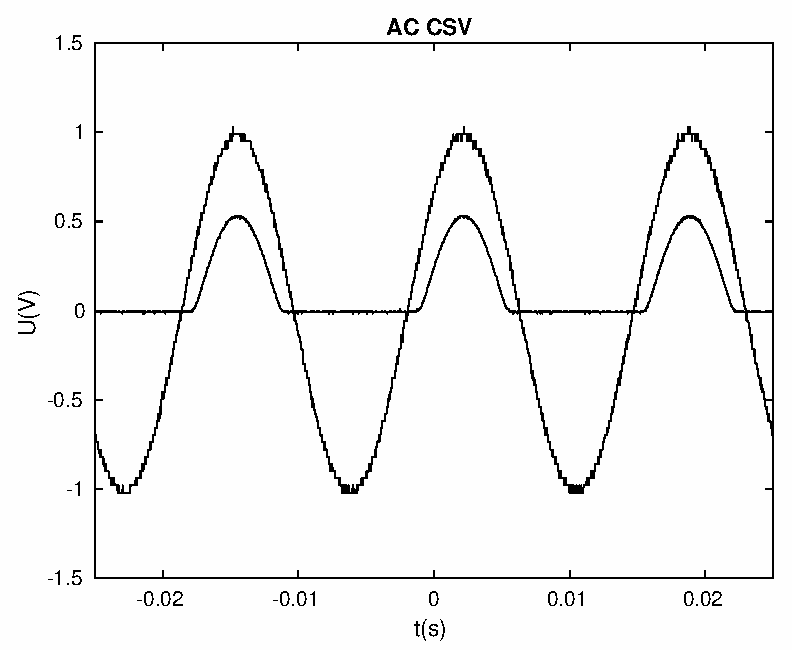
\includegraphics[width=0.7\linewidth]{imgs/ac-csv.eps}
	\caption{Curve of the csv file}
	\label{fig-2-1}
\end{figure}

With the following equation:
$$I_d=\frac{V_0-V_d}{R}$$

The I-V curve of the diode can be shown in Figure \ref{fig-2-2}.

\begin{figure}[!htbp]
	\centering
	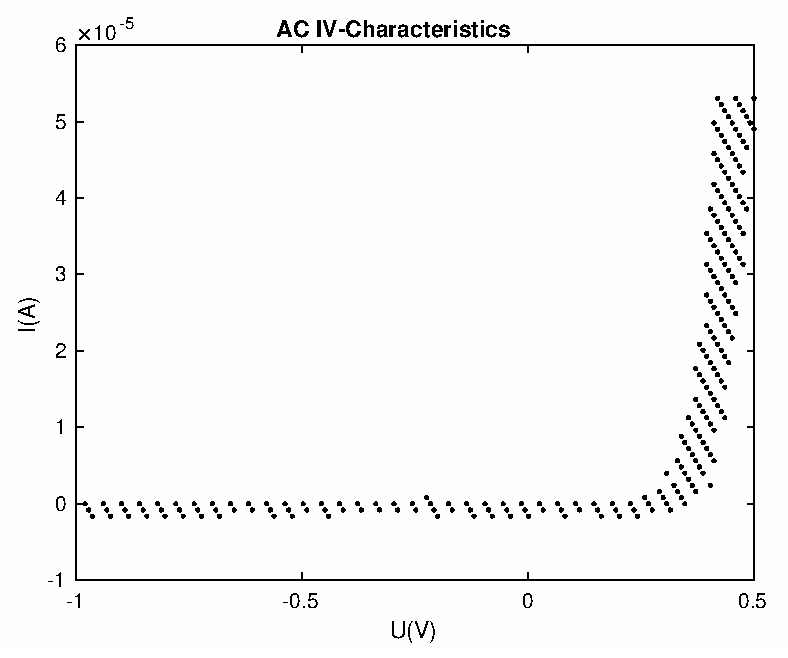
\includegraphics[width=0.7\linewidth]{imgs/ac-iv.eps}
	\caption{AC IV-Characteristics}
	\label{fig-2-2}
\end{figure}


\newpage

According to the curve, the value of $V_{on}$ is around 0.5$V$.

\subsubsection{DC analysis}
In DC part, we input DC signal whose voltage ranges from 0 to 1$V$. By measuring the voltage of the diode, we successfully got  Table \ref{tab-2} 

\begin{table}[!htbp]
    \centering
    \begin{tabular}{|c|c|}
    \hline
    DC Voltage (V) & Resistance Voltage (mV) \\\hline
    1	&   540.5   \\\hline
    0.9	&   538     \\\hline
    0.8	&   530.5   \\\hline
    0.7	&   525     \\\hline
    0.6	&   501     \\\hline
    0.5	&   478.5   \\\hline
    0.4	&   394.5   \\\hline
    0.3	&   292     \\\hline
    0.2	&   193     \\\hline
    0.1	&   90.5    \\\hline
    \end{tabular}
    \caption{DC measurement of diode.}
    \label{tab-2}
\end{table}

Then the I-V character of diode was shown in Figure \ref{fig-2-3}

\begin{figure}[!htbp]
	\centering
	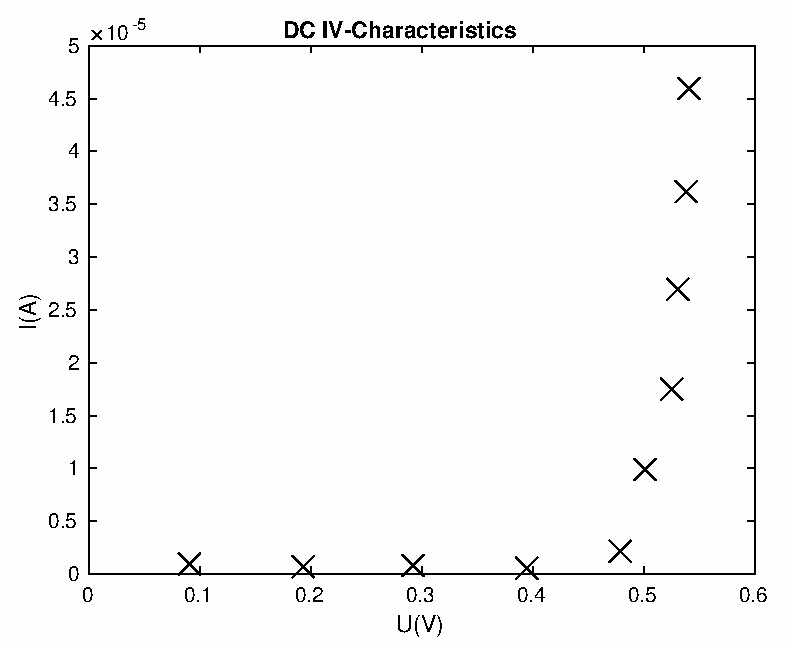
\includegraphics[width=0.7\linewidth]{imgs/dc-iv.eps}
	\caption{DC IV-Characteristics}
	\label{fig-2-3}
\end{figure}

\newpage
According to the graph, the $V_on$ is around 0.5$V$,which corresponding to the value we get in the AC part.

\subsection{Back-to-back diodes}

In Pspice, we simulate the behavior of two diodes which is connected back to back under different amplitudes, which was shown in Figure \ref{fig-3-1}, Figure \ref{fig-3-2}, Figure \ref{fig-3-3} and Figure \ref{fig-3-4}.

The chosen diode is D1N4148.

\begin{figure}[!htbp]
	\centering
	\subfigure[Voltage]{\includegraphics[width=0.45\linewidth]{imgs/b2b1_v.png}}
	\subfigure[Current]{\includegraphics[width=0.45\linewidth]{imgs/b2b1_i.png}}
	\caption{1 Vpp Back-to-back diodes}
	\label{fig-3-1}
\end{figure}

\begin{figure}[!htbp]
	\centering
	\subfigure[Voltage]{\includegraphics[width=0.45\linewidth]{imgs/b2b2_v.png}}
	\subfigure[Current]{\includegraphics[width=0.45\linewidth]{imgs/b2b2_i.png}}
	\caption{2 Vpp Back-to-back diodes}
	\label{fig-3-2}
\end{figure}

\begin{figure}[!htbp]
	\centering
	\subfigure[Voltage]{\includegraphics[width=0.45\linewidth]{imgs/b2b5_v.png}}
	\subfigure[Current]{\includegraphics[width=0.45\linewidth]{imgs/b2b5_i.png}}
	\caption{5 Vpp Back-to-back diodes}
	\label{fig-3-3}
\end{figure}

\begin{figure}[!htbp]
	\centering
	\subfigure[Voltage]{\includegraphics[width=0.45\linewidth]{imgs/b2b10_v.png}}
	\subfigure[Current]{\includegraphics[width=0.45\linewidth]{imgs/b2b10_i.png}}
	\caption{10 Vpp Back-to-back diodes}
	\label{fig-3-4}
\end{figure}

\newpage
\subsection{Face-to-face diodes}
We simulate the behavior of two diodes connected face to face under different amplitudes, which was shown in Figure \ref{fig-4-1}, Figure \ref{fig-4-2}, Figure \ref{fig-4-3} and Figure \ref{fig-4-4}.

\begin{figure}[!htbp]
	\centering
	\subfigure[Voltage]{\includegraphics[width=0.45\linewidth]{imgs/f2f1_v.png}}
	\subfigure[Current]{\includegraphics[width=0.45\linewidth]{imgs/f2f1_i.png}}
	\caption{1 Vpp Face-to-face diodes}
	\label{fig-4-1}
\end{figure}

\begin{figure}[!htbp]
	\centering
	\subfigure[Voltage]{\includegraphics[width=0.45\linewidth]{imgs/f2f2_v.png}}
	\subfigure[Current]{\includegraphics[width=0.45\linewidth]{imgs/f2f2_i.png}}
	\caption{2 Vpp Face-to-face diodes}
	\label{fig-4-2}
\end{figure}

\begin{figure}[!htbp]
	\centering
	\subfigure[Voltage]{\includegraphics[width=0.45\linewidth]{imgs/f2f5_v.png}}
	\subfigure[Current]{\includegraphics[width=0.45\linewidth]{imgs/f2f5_i.png}}
	\caption{5 Vpp Face-to-face diodes}
	\label{fig-4-3}
\end{figure}

\begin{figure}[!htbp]
	\centering
	\subfigure[Voltage]{\includegraphics[width=0.45\linewidth]{imgs/f2f10_v.png}}
	\subfigure[Current]{\includegraphics[width=0.45\linewidth]{imgs/f2f10_i.png}}
	\caption{10 Vpp Face-to-face diodes}
	\label{fig-4-4}
\end{figure}

\newpage
\section{Conclusion}

In the first part, we measured the turning on voltage of the diode. According to the calculation, its value is 0.74V, which is corresponding to our estimation about 0.6-0.7$V$.


We analyze the I-V character of diode in the second section. With both AC input and DC input, we get the same value of $V_on$ which is around 0.5V. Though the shape of the graph correspond to the expected I-V character of the diode, the value is smaller than the result in the first part. The problem might be the resistance of the machine and the multimeter. Since we directly apply the value of the input voltage instead of measuring the voltage of the two end of the circuit, some error will occur during the calculation.

The third part measures the behaviour of two face-to-face and back-to-back diodes. As shown in the graph, the shape of current graph is a bit wield. We tried to get its character under DC input, which was shown in Figure \ref{fig-conclusion}.

\begin{figure}[!htbp]
	\centering
	\includegraphics[width=0.7\linewidth]{imgs/conclusion.png}
	\caption{DC IV-Characteristics of Face-to-face diodes}
	\label{fig-conclusion}
\end{figure}

The simulation results indicate that the working voltage of face-to-face circuit becomes extremely large which is equal to the reverse breakdown voltage of the diode. As a result, the value of the current becomes very small. The increasing and decreasing part of the current is almost the same as sine wave. The resistance changing of the two diodes system causes the wield shape of the current flow. 



\newpage

\section{Reference}

\subsection{References}
\begin{enumerate}
	\item Lab2 Manual
\end{enumerate}

\subsection{Matlab Code}
\vspace*{1em}

\begin{minipage}{0.1\linewidth}
\end{minipage}
\begin{minipage}{0.8\linewidth}
    \inputminted{matlab}{p2.m}
\end{minipage}

\end{document}
